\documentclass[pra, onecolumn, notitlepage, floats, 11pt]{revtex4-1}

\usepackage[T1]{fontenc}
\usepackage{graphicx}
\usepackage{color}
\usepackage{latexsym,amsmath}
\usepackage{comment}
\usepackage{tabularx}
\usepackage{siunitx}
\usepackage{multirow}
\usepackage{mathtools}
\usepackage{tikz, fp}
\usepackage{wrapfig}
\usepackage{amsfonts}
\usepackage[pdftex,colorlinks=true, pdfstartview=FitV, linkcolor=linkcolor, citecolor=linkcolor, urlcolor=linkcolor, hyperindex=true,hyperfigures=true]{hyperref} %hyperlink%
\usepackage{fancyhdr}
\usepackage{inconsolata}
\usepackage{listings}
\usepackage{physics}
\usepackage{datetime}
\usepackage[caption=false]{subfig}
\usepackage{titlesec}

\renewcommand{\figurename}{Figure}
\renewcommand{\tablename}{Table}
\renewcommand{\thetable}{\arabic{table}}

\definecolor{airforceblue}{rgb}{0.36, 0.54, 0.66}  %#5D8AA8
\definecolor{cobalt}{rgb}{0.0, 0.28, 0.67}         %#0047AB
\definecolor{coolblack}{rgb}{0.0, 0.18, 0.39}      %#002E63
\definecolor{dartmouthgreen}{rgb}{0.05, 0.5, 0.06} %#00693E
\definecolor{mydmg}{rgb}{0.05, 0.5, 0.06}          %#00693E
\definecolor{lava}{rgb}{0.81, 0.06, 0.13}          %#CF1020
\definecolor{myred}{rgb}{0.81, 0.06, 0.13}         %#CF1020
% move section headings to left
% \sffamily
% \scshape
%\titleformat{\section}{\raggedright\sffamily\bfseries\fontsize{13pt}{13}\selectfont}{\arabic{section}}{1em}{\MakeUppercase}
\titleformat{\section}{\raggedright\bfseries\scshape\fontsize{13pt}{13}\selectfont}{\color{cobalt}\arabic{section}}{1em}{\color{cobalt}}
\titleformat{\subsection}{\raggedright\bfseries\scshape\fontsize{12pt}{12}\selectfont}{{\color{cobalt}\arabic{section}.\arabic{subsection}}}{1em}{\color{cobalt}}
\renewcommand{\thesection}{\arabic{section}}
\renewcommand{\thesubsection}{\arabic{subsection}}
\renewcommand{\thesubsubsection}{\arabic{subsubsection}}
\makeatletter
\renewcommand{\p@subsection}{\thesection.}
\renewcommand{\p@subsubsection}{\thesection.\thesubsection.}
\makeatother


\linespread{0.956}

\DeclarePairedDelimiter\ceil{\lceil}{\rceil}
\DeclarePairedDelimiter\floor{\lfloor}{\rfloor}

\definecolor{linkcolor}{rgb}{0,0,0.65}
\definecolor{shadecolor}{rgb}{0.95, 0.95, 0.95}
\definecolor{mygreen}{rgb}{0,0.6,0}
\definecolor{mygray}{rgb}{0.5,0.5,0.5}
\definecolor{mymauve}{rgb}{0.58,0,0.82}
\lstdefinestyle{fortran}
{
    backgroundcolor=\color{shadecolor},       % background color
    basicstyle=\ttfamily\scriptsize,          % the size of the fonts that are used for the code
    breakatwhitespace=false,                  % sets if automatic breaks should only happen at whitespace
    breaklines=false,                         % sets automatic line breaking
    captionpos=b,                             % sets the caption-position to bottom
    commentstyle=\color{mygreen},             % comment style
    extendedchars=true,                       % lets you use non-ASCII characters; for 8-bits encodings only, does not work with UTF-8
    keepspaces=true,                          % keeps spaces in text, useful for keeping indentation of code (possibly needs columns=flexible)
    keywordstyle=\bfseries\color{blue},       % keyword style
    language=[95]Fortran,                     % the language of the code
    numbers=left,                             % where to put the line-numbers; possible values are (none, left, right)
    numbersep=5pt,                            % how far the line-numbers are from the code
    numberstyle=\tiny\color{mygray},          % the style that is used for the line-numbers
    rulecolor=\color{black},                  % if not set, the frame-color may be changed on line-breaks within not-black text (e.g. comments (green here))
    showspaces=false,                         % show spaces everywhere adding particular underscores; it overrides 'showstringspaces'
    showstringspaces=false,                   % underline spaces within strings only
    showtabs=false,                           % show tabs within strings adding particular underscores
    stepnumber=1,                             % the step between two line-numbers. If it's 1, each line will be numbered
    stringstyle=\color{mymauve},              % string literal style
    tabsize=4,                                % sets default tabsize to 4 spaces
    title=\lstname                            % show the filename of files
}

\lstdefinestyle{python}
{
    backgroundcolor=\color{shadecolor},       % background color
    basicstyle=\ttfamily\scriptsize,          % the size of the fonts that are used for the code
    breakatwhitespace=false,                  % sets if automatic breaks should only happen at whitespace
    breaklines=false,                         % sets automatic line breaking
    captionpos=b,                             % sets the caption-position to bottom
    commentstyle=\color{mygreen},             % comment style
    extendedchars=true,                       % lets you use non-ASCII characters; for 8-bits encodings only, does not work with UTF-8
    keepspaces=true,                          % keeps spaces in text, useful for keeping indentation of code (possibly needs columns=flexible)
    keywordstyle=\bfseries\color{blue},       % keyword style
    language=Python,                          % the language of the code
    numbers=left,                             % where to put the line-numbers; possible values are (none, left, right)
    numbersep=5pt,                            % how far the line-numbers are from the code
    numberstyle=\tiny\color{mygray},          % the style that is used for the line-numbers
    rulecolor=\color{black},                  % if not set, the frame-color may be changed on line-breaks within not-black text (e.g. comments (green here))
    showspaces=false,                         % show spaces everywhere adding particular underscores; it overrides 'showstringspaces'
    showstringspaces=false,                   % underline spaces within strings only
    showtabs=false,                           % show tabs within strings adding particular underscores
    stepnumber=1,                             % the step between two line-numbers. If it's 1, each line will be numbered
    stringstyle=\color{mymauve},              % string literal style
    tabsize=4,                                % sets default tabsize to 4 spaces
    title=\lstname                            % show the filename of files
}

\lstdefinestyle{bash}
{
    backgroundcolor=\color{shadecolor},       % background color
    basicstyle=\ttfamily\scriptsize,          % the size of the fonts that are used for the code
    breakatwhitespace=false,                  % sets if automatic breaks should only happen at whitespace
    breaklines=false,                         % sets automatic line breaking
    captionpos=b,                             % sets the caption-position to bottom
    commentstyle=\color{mygreen},             % comment style
    extendedchars=true,                       % lets you use non-ASCII characters; for 8-bits encodings only, does not work with UTF-8
    keepspaces=true,                          % keeps spaces in text, useful for keeping indentation of code (possibly needs columns=flexible)
    keywordstyle=\bfseries\color{blue},       % keyword style
    language=bash,                            % the language of the code
    numbers=left,                             % where to put the line-numbers; possible values are (none, left, right)
    numbersep=5pt,                            % how far the line-numbers are from the code
    numberstyle=\tiny\color{mygray},          % the style that is used for the line-numbers
    rulecolor=\color{black},                  % if not set, the frame-color may be changed on line-breaks within not-black text (e.g. comments (green here))
    showspaces=false,                         % show spaces everywhere adding particular underscores; it overrides 'showstringspaces'
    showstringspaces=false,                   % underline spaces within strings only
    showtabs=false,                           % show tabs within strings adding particular underscores
    stepnumber=1,                             % the step between two line-numbers. If it's 1, each line will be numbered
    stringstyle=\color{mymauve},              % string literal style
    tabsize=4,                                % sets default tabsize to 4 spaces
    title=\lstname                            % show the filename of files
}

\makeatletter
\newcommand{\srcsize}{\@setfontsize{\srcsize}{5pt}{5pt}}
\makeatother


\pagestyle{fancy}
\fancyhf{}
\fancyhead[L]{Rocco Ardino (Mat. 1231629)}
\fancyhead[R]{\bf\thepage}
\fancyfoot[L]{\textsc{report}: Week 8}
\fancyfoot[R]{\today}
\renewcommand{\headrulewidth}{0.1pt}
\renewcommand{\footrulewidth}{0.1pt}

\newcommand{\codebold}[2][cobalt]{\texttt{\bfseries {\color{#1}#2}}}
\newcommand{\code}[2][black]{\color{#1}\texttt{#2}}
\newcommand{\codefunctionbold}[2]{\texttt{\bfseries {\color{cobalt}#1}({\color{lava}#2})}}
\newcommand{\codefunction}[2]{\texttt{#1(#2})}










\begin{document}

\title{Quantum Information and Computing 2020/21\\Week 8 report}

\author{Rocco Ardino}

\date{\today}





\begin{abstract}
    In this work we deal with quantum \( N \)-body states and density matrices. We first face the problem of a minimal memory consuming description of those states in both separable and non-separable cases. Then, we implement the initialization of the density matrix from a certain wavefunction and the partial trace operation, performed on a certain subsystem. Lastly, we test everything on a system of 2 qubits.
\end{abstract}

\maketitle





\section{Theory}
Let us consider a quantum \( N \)-body system, where each subsystem wavefunction is denoted by \( \ket{\psi_{i}} \in \mathcal{H}^{d} \). Without losing of generality, it is convenient to write each \( \ket{\psi_{i}} \) as a linear combination of \( \ket{\alpha_{j}} \in \qty{\ket{0},\dots,\ket{d-1}} \).
Therefore, with this notation, the wavefunction \( \ket{\Psi} \in \mathcal{H}^{d^{N}} \) of the whole pure state system reads:
\begin{equation}
    \ket{\Psi}
    =
    \sum_{\alpha_{1},\dots,\alpha_{N}}
    C_{\alpha_{1},\dots,\alpha_{N}}
    \ket{\alpha_{1}}
    \otimes
    \cdots
    \otimes
    \ket{\alpha_{N}}
    \quad ,
    \label{eq:08_T_1}
\end{equation}
with \( C_{\alpha_{1},\dots,\alpha_{N}} \) complex coefficients. Another way to express Eq. \ref{eq:08_T_1}, which exploits the \( d \)-basis representation and which will be useful for the code implementation, reads:
\begin{equation}
    \ket{\Psi}
    =
    \sum_{i=0}^{d^{N}-1} C_{i} \ket{i}
    \quad , \quad
    i
    =
    \sum_{j=1}^{N} \alpha_{j} d^{j-1}
    \quad .
    \label{eq:08_T_2}
\end{equation}

A special case of the previous discussion is the one of a separable pure state. In this case the \( N \)-body wavefunction has a simpler form:
\begin{equation}
    \ket{\Psi}
    =
    \qty(\sum_{\alpha_{1}} C_{\alpha_{1}} \ket{\alpha_{1}})
    \otimes
    \cdots
    \otimes
    \qty(\sum_{\alpha_{N}} C_{\alpha_{N}} \ket{\alpha_{N}})
    \quad
    .
    \label{eq:08_T_3}
\end{equation}
We can see the difference with the non-separable case. In fact, the ladder is defined by \( d^{N} \) complex coefficients, while the separable wavefunction requires \( d \cdot N \) complex coefficients. This fact translates in a significantly smaller initialization time for a separable wave function.

After having determined the pure state \( N \)-body wavefunction \( \ket{\Psi} \), its density matrix is defined as follows:
\begin{equation}
    \rho
    =
    \ket{\Psi} \bra{\Psi}
    =
    \sum_{i,j=0}^{d^{N}-1} C^{*}_{j} C_{i} \ket{i} \bra{j}
    \quad .
    \label{eq:08_T_4}
\end{equation}
Starting from this definition, a reduced density matrix on the \( k^{\text{th}} \) subsystem is computed by tracing over all the remaining subsystems:
\begin{equation}
    \rho_{k}
    =
    \tr_{1} \cdots \tr_{k-1} \tr_{k+1} \cdots \tr_{N} \rho
    \quad ,
    \label{eq:08_T_5}
\end{equation}
where the trace with index \( i \) reads:
\begin{equation}
    \tr_{i} \rho
    =
    \sum_{j=0}^{d-1} \expval{\rho}{j}
    \quad .
    \label{eq:08_T_6}
\end{equation}





\section{Code Development}
For this work, the new module \codebold{dmat} is implemented, containing several functions and subroutines for multiple purposes:
\vspace{-5pt}
\begin{itemize}%[nolistsep]
    \setlength\itemsep{-3pt}
    \item \codefunctionbold{dmat\_init\_rand\_state}{N,D,isSep}, for instantiating a \( N \)-body (non-)separable system, with each subsystem living inside \( \mathcal{H}^{d} \);
    \item \codefunctionbold{dmat\_init\_rho}{state}, for initializing the density matrix, given the state;
    \item \codefunctionbold{dmat\_rho\_reduce}{rho,nsub,N,D}, for calculating the reduced density matrix, obtained by tracing the \( \code{nsub} \) subsystem;
    \item \codefunctionbold{dmat\_print\_state\_std}{state,formatted}, for printing the state coefficients on standard output and in a formatted way, if specified;
    \item \codefunctionbold{dmat\_print\_rho\_std}{rho,formatted}, for printing the density matrix entries on standard output and in a formatted way, if specified.
\end{itemize}

Moreover, another module, namely \codebold{cmdline}, is implemented to have a command-line argument parser and for default arguments handling. In particular, we explain the new core functionalities of both the modules in the following subsections.



\subsection{Pure state initialization}
The code to perform the initialization of the state coefficients is showed in Listing \ref{lst:08_C_SS_1_1}. Note how the operation is vectorized through the intrinsic function \code{RANDOM\_NUMBER} and the difference in the number of coefficients depending on the separability of the state.

\medskip
\begin{lstlisting}[
    style=fortran,
    frame=single,
    label={lst:08_C_SS_1_1},
    caption={Implementation of the state coefficients initialization.}
]
function dmat_init_rand_state(N, D, isSep) result(state)
    ! input arguments
    integer(4) :: N
    integer(4) :: D
    logical    :: isSep

    integer(4) :: dim
    complex(8), dimension(:), allocatable :: state
    real(8),    dimension(:), allocatable :: re, im
    real(8)    :: norm

    if (isSep) then
        dim = D*N
    else
        dim = D**N
    end if

    allocate(state(dim))
    allocate(re(dim))
    allocate(im(dim))

    ! fill real and imaginary part vectors
    call RANDOM_NUMBER(re)
    call RANDOM_NUMBER(im)
    re = re*2.0d0 - 1.0d0
    im = im*2.0d0 - 1.0d0

    ! fill state vector with coefficients and normalize
    norm  = SUM(re**2 + im**2)
    state = (re*COMPLEX(1.0d0,0.0d0) + im*COMPLEX(0.0d0,1.0d0)) / COMPLEX(SQRT(norm),0.0d0)
end function dmat_init_rand_state
\end{lstlisting}



\subsection{Density matrix initialization}
The code to perform the the initialization of the density matrix is showed in Listing \ref{lst:08_C_SS_2_1}. The technique employed is nothing more than a tensor product, performed using the intrinsic \code{MATMUL}. At the end of the execution, the apposite function returns a \( d^{N} \times d^{N} \) complex matrix.

\medskip
\begin{lstlisting}[
    style=fortran,
    frame=single,
    label={lst:08_C_SS_2_1},
    caption={Implementation of the density matrix initialization.}
]
function dmat_init_rho(state) result(rho)
    ! input arguments
    complex(8), dimension(:) :: state

    complex(8), dimension(:,:), allocatable :: rho
    complex(8), dimension(:,:), allocatable :: bra, ket
    integer(4) :: N

    N = size(state,1)

    allocate(rho(N,N))
    allocate(bra(1,N))
    allocate(ket(N,1))

    bra(1,:) = CONJG(state)
    ket(:,1) =       state

    rho = MATMUL(ket,bra)
end function dmat_init_rho
\end{lstlisting}



\subsection{Density matrix reduction}
The code to perform the reduction of density matrix, by tracing on the \( k^{\text{th}} \) subsystem, is showed in Listing \ref{lst:08_C_SS_3_1}. What is important to observe is that the technique of using a \( d \)-basis representation of Eq. \ref{eq:08_T_2} is employed. If we consider a number written in this representation, with the \( \alpha_{i} \)s representing its digits, we need two loops for every dimension of the density matrix:
\begin{itemize}
    \setlength\itemsep{-3pt}
    \item one for cycling over the less significant \( \alpha_{i} \)s, namely the ones with \( i < k \);
    \item one for cycling over the more significant \( \alpha_{i} \)s, namely the ones with \( i > k \).
\end{itemize}
Then, another loop over \( \alpha_{k} \) is needed in order to perform the summations needed for the trace.

\medskip
\begin{lstlisting}[
    style=fortran,
    frame=single,
    label={lst:08_C_SS_3_1},
    caption={Implementation of the function for density matrix reduction over the \( k^{\text{th}} \) subsystem.}
]
function dmat_rho_reduce(rho, nsub, N, D) result(rho_red)
    ! input arguments
    complex(8), dimension(:,:) :: rho
    integer(4) :: nsub
    integer(4) :: N
    integer(4) :: D

    complex(8), dimension(D**(N-1),D**(N-1)) :: rho_red
    complex(8) :: sum
    integer(4) :: lli, llj, mmi, mmj, kk, ii, jj, iir, jjr

    ! loop over rho elements of all subsystems except nsub
    do lli=0,D**(nsub-1)-1
        do mmi=0,(D**(N-nsub))-1
            do llj=0,D**(nsub-1)-1
                do mmj=0,(d**(N-nsub))-1
                    ! trace the nsub subsystem
                    sum = COMPLEX(0.0d0,0.0d0)
                    do kk=0,D-1
                        ii = lli + 1 + (kk + mmi*D)*D**(nsub-1)
                        jj = llj + 1 + (kk + mmj*D)*D**(nsub-1)
                        sum = sum + rho(ii,jj)
                    end do
                    ! fill reduced density matrix
                    iir = lli + 1 + mmi*D**(nsub-1)
                    jjr = llj + 1 + mmj*D**(nsub-1)
                    rho_red(iir, jjr) = sum
                end do
            end do
        end do
    end do
end function dmat_rho_reduce
\end{lstlisting}



\subsection{Main program}
Lastly, all the functions described before are employed in a main program, in which a command-line argument parser is implemented in order to obtain an easier handling of the parameters of the simulation. Moreover, this functionality is also capable of giving default values to the arguments when they are not given.
To make the program more user-friendly, a \code{-h} help option has been added and in the beginning of the execution all the arguments given are printed along with a flag: \codebold[red]{F} if a value is given for it, \codebold[dartmouthgreen]{T} if default is taken. An example of this functionality and of the way to start the program is showed in Listing \ref{lst:08_C_SS_4_1}. A complete list of the options is given in Table \ref{tab:08_C_SS_4_1}.

\begin{table}[!h]
\begin{minipage}[t]{0.48\textwidth}
    \raisebox{-\height}{
    {\footnotesize
    \begin{tabular}{cccc}
        \toprule
        Arg option    &   Arg name        &   Arg meaning   &   Default     \\
        \colrule
        \code{-N}    &   \code{subsysN}     &   \( N \)             &   \( 2 \) \\
        \code{-D}    &   \code{dimD}        &   \( d \)             &   \( 2 \) \\
        \code{-S}    &   \code{separable}   &   Separability        &   \( 0 \) \\
        \code{-M}    &   \code{mode}        &   Execution routine   &   \( 1 \) \\
        \code{-K}    &   \code{reduceK}     &   Subsystem to reduce &   \( 1 \) \\
        \code{-h}    &   \code{help}        &   print help          &           \\
        \botrule
    \end{tabular}
    }}
    \caption{Command-line arguments of the program.}
    \label{tab:08_C_SS_4_1}
\end{minipage}
\hfill
\begin{minipage}[t]{0.48\textwidth}
\begin{lstlisting}[
    style=bash,
    frame=single,
    escapechar=!,
    label={lst:08_C_SS_4_1},
    caption={Example of launch and user interface.}
]
!{\bfseries\color{dartmouthgreen}\$}! !{\bfseries\color{cobalt}./08.o}! !{\bfseries\color{lava}-S}! 0 !{\bfseries\color{lava}-M}! 1

Running with the following cmdline options:

N =	       2	default [T/F]: !{\bfseries\color{dartmouthgreen}T}!
D =	       2	default [T/F]: !{\bfseries\color{dartmouthgreen}T}!
S =	       0	default [T/F]: !{\bfseries\color{red}F}!
M =	       1	default [T/F]: !{\bfseries\color{red}F}!
K =	       1	default [T/F]: !{\bfseries\color{dartmouthgreen}T}!

CPU time:
3.1999999999999910E-005
\end{lstlisting}
\end{minipage}
\end{table}

After the parser, if no exception is found, a subroutine with the corresponding mode of execution is called. The possible modes are the following:
\begin{itemize}
    \setlength\itemsep{-3pt}
    \item \codebold[black]{mode\_1}: it executes state initialization and returns CPU time needed for the purpose;
    \item \codebold[black]{mode\_2}: it executes state and density matrix initialization (only for non-separable states), reduces by tracing on the \( k^{\text{th}} \) subsystem and prints both \( \rho \) and reduced \( \rho \);
    \item \codebold[black]{mode\_3}: it does the same operations as \code{mode\_2}, but with a system of two spin one-half qubits and with reduction of both subsytems.
\end{itemize}

Last but not least, the program must be compiled with the flag \code{-ffree-line-length-0}.





\section{Results}



\subsection{State initialization efficiency}
The first analysis performed concerns the CPU time needed to initialize a fully defined \( N \)-body pure state for both separable and non-separable cases. For this purpose, the code returning the CPU time is run for multiple combinations of \( N \) and \( d \). The results are showed in Figure \ref{fig:08_R_SS_1}. What is important to remark is how, fixed \( d \), the CPU time needed for the initialization of a separable state is polynomial in \( N \), while it is exponential in \( N \) for the non-separable case. This is what we expect if we think in terms of the number of coefficients needed.

\begin{figure}[!h]
    \centering
    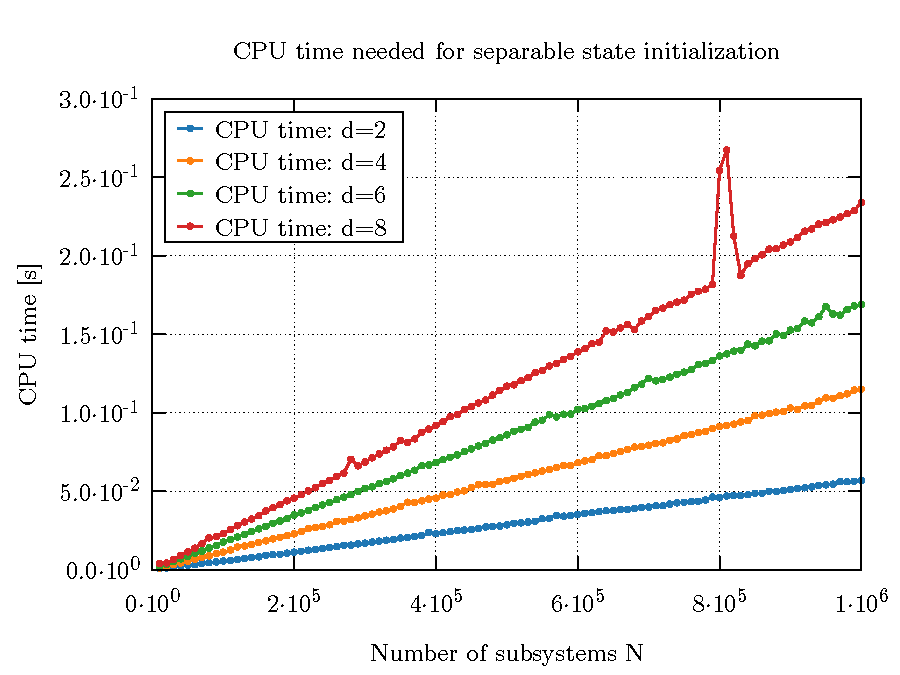
\includegraphics[width=0.32\textwidth]{images/separable.pdf}
    \hfill
    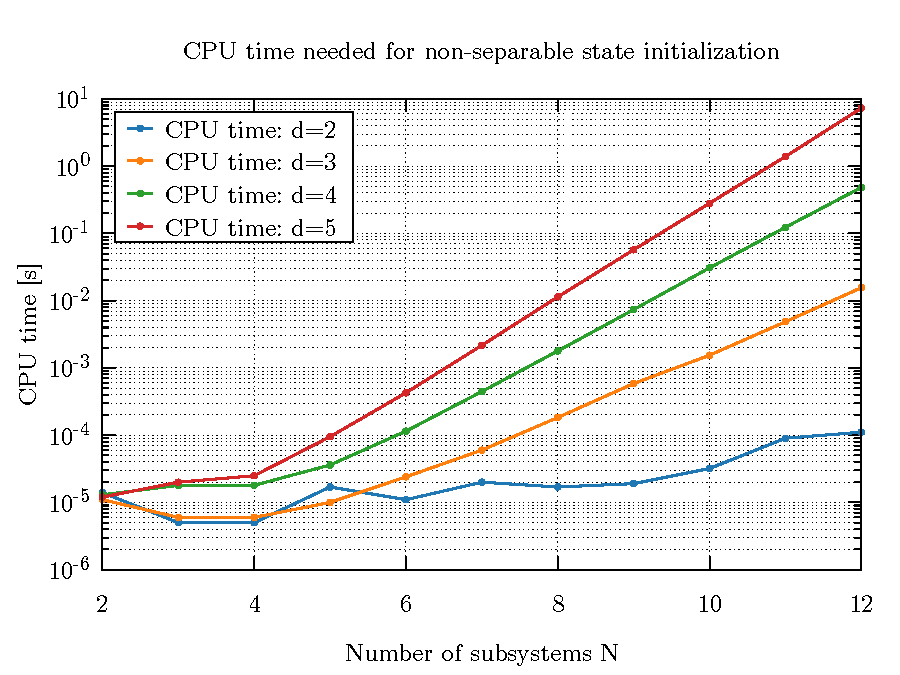
\includegraphics[width=0.32\textwidth]{images/nonseparable.pdf}
    \hfill
    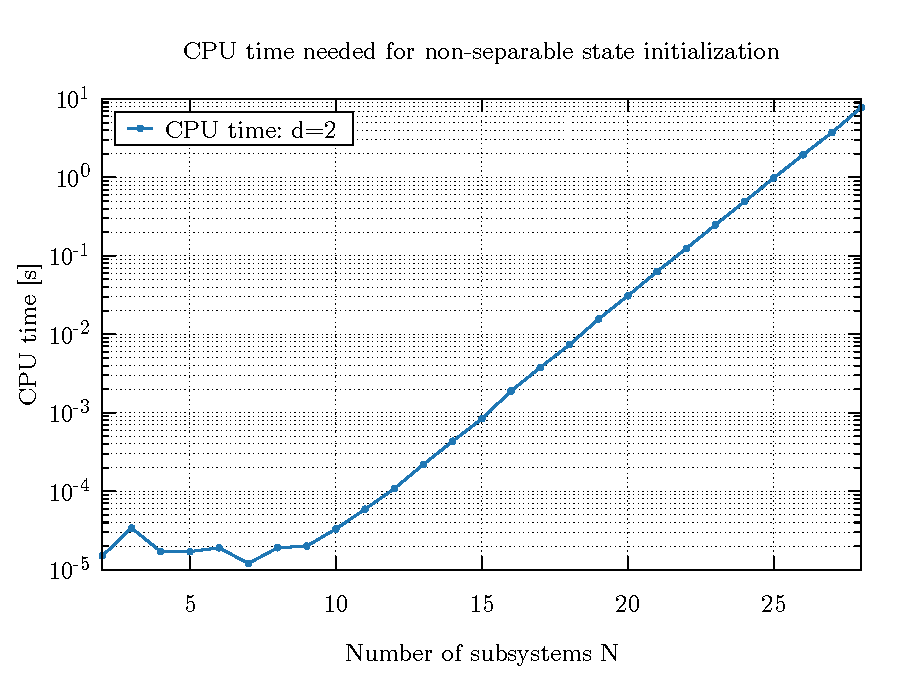
\includegraphics[width=0.32\textwidth]{images/nonseparable_2.pdf}
    \caption{\label{fig:08_R_SS_1} CPU time results for separable (left) and non-separable (center) state initialization, depending on \( N \) and \( d \), and for a non-separable state initialization with fixed \( d=2 \) and larger values of \( N \) (right).}
\end{figure}



\subsection{Density matrix calculation and reduction for \( N = 2 \), \( d = 2 \)}
The code implementation for density matrix initialization and reduction is validated for \( N = d = 2 \), namely for the case of two spin one-half qubits. The execution mode 3 is run for several cases and an example result is showed in Listing \ref{lst:08_R_SS_2_1}. The ladder shows the correctness of the partial tracing operation implemented.

\medskip
\begin{lstlisting}[
    style=bash,
    frame=single,
    escapechar=!,
    % basicstyle=\ttfamily\tiny,
    label={lst:08_R_SS_2_1},
    caption={Example of execution for two spin one-half qubits, with density matrix initialization and reduction.}
]
!{\bfseries\color{dartmouthgreen}\$}! !{\bfseries\color{cobalt}./08.o}! !{\bfseries\color{lava}-M}! 3

!{\color{black}Running for two spin one-half qubits:}!

!{\color{black}State coefficients:}!
!{\bfseries\color{black}(-0.3267 -0.4480i)}!
!{\bfseries\color{black}( 0.0629 +0.6569i)}!
!{\bfseries\color{black}( 0.4124 -0.1932i)}!
!{\bfseries\color{black}(-0.1970 +0.1043i)}!

!{\color{black}Density matrix:}!
!{\bfseries\color{myred}( 0.3074 +0.0000i)}! !{\bfseries\color{black}(-0.3148 +0.1864i)}! !{\bfseries\color{black}(-0.0482 -0.2479i)}! !{\bfseries\color{black}( 0.0176 +0.1223i)}!
!{\bfseries\color{black}(-0.3148 -0.1864i)}! !{\bfseries\color{myred}( 0.4355 -0.0000i)}! !{\bfseries\color{black}(-0.1010 +0.2830i)}! !{\bfseries\color{black}( 0.0561 -0.1360i)}!
!{\bfseries\color{black}(-0.0482 +0.2479i)}! !{\bfseries\color{black}(-0.1010 -0.2830i)}! !{\bfseries\color{myred}( 0.2074 +0.0000i)}! !{\bfseries\color{black}(-0.1014 -0.0049i)}!
!{\bfseries\color{black}( 0.0176 -0.1223i)}! !{\bfseries\color{black}( 0.0561 +0.1360i)}! !{\bfseries\color{black}(-0.1014 +0.0049i)}! !{\bfseries\color{myred}( 0.0497 +0.0000i)}!

!{\color{black}Reduced density matrix (on left system):}!
!{\bfseries\color{myred}( 0.7429 +0.0000i)}! !{\bfseries\color{black}( 0.0080 -0.3839i)}!
!{\bfseries\color{black}( 0.0080 +0.3839i)}! !{\bfseries\color{myred}( 0.2571 +0.0000i)}!

!{\color{black}Reduced density matrix (on right system):}!
!{\bfseries\color{myred}( 0.5148 +0.0000i)}! !{\bfseries\color{black}(-0.4162 +0.1815i)}!
!{\bfseries\color{black}(-0.4162 -0.1815i)}! !{\bfseries\color{myred}( 0.4852 -0.0000i)}!
\end{lstlisting}


\section{Self-evaluation}
In this work we have faced the problem of density matrices initialization and handling, as well as pure state definition efficiency for both separable and non-separable cases. The code implementation has led to successful results for the density matrix initialization and partial tracing, validated with the example of 2 qubits. Moreover, it has showed the efficiency of state coefficients initialization for different values of \( N \) and \( d \).

\end{document}
